\documentclass[10pt,twocolumn,letterpaper]{article}

\usepackage{cvpr}
\usepackage{times}
\usepackage{epsfig}
\usepackage{graphicx}
\usepackage{amsmath}
\usepackage{amssymb}

% Include other packages here, before hyperref.

\usepackage[breaklinks=true,bookmarks=false]{hyperref}

\cvprfinalcopy

\def\httilde{\mbox{\tt\raisebox{-.5ex}{\symbol{126}}}}

\begin{document}

\title{Geneus: An Enigma of Organism Intelligence}

\author{Jason Dong, Yidi Huang, Mark Lalor, Andrew Tarnoff, Hung Vu \\
Case Western Reserve University\\
10900 Euclid Ave, Cleveland, OH 44106\\
{\tt\small jwd67@case.edu, yxh597@case.edu, mwl58@case.edu, art81@case.edu, hdv4@case.edu}}

\maketitle

\begin{abstract}
   This will be teh abstract which will be wonderfully descriptive yet succinct.
\end{abstract}

\section{Introduction}

This is the introduction \cite{Alpher02}

\section{Background}

This is the background \cite{Alpher04}

\section{Data}

\begin{figure}
  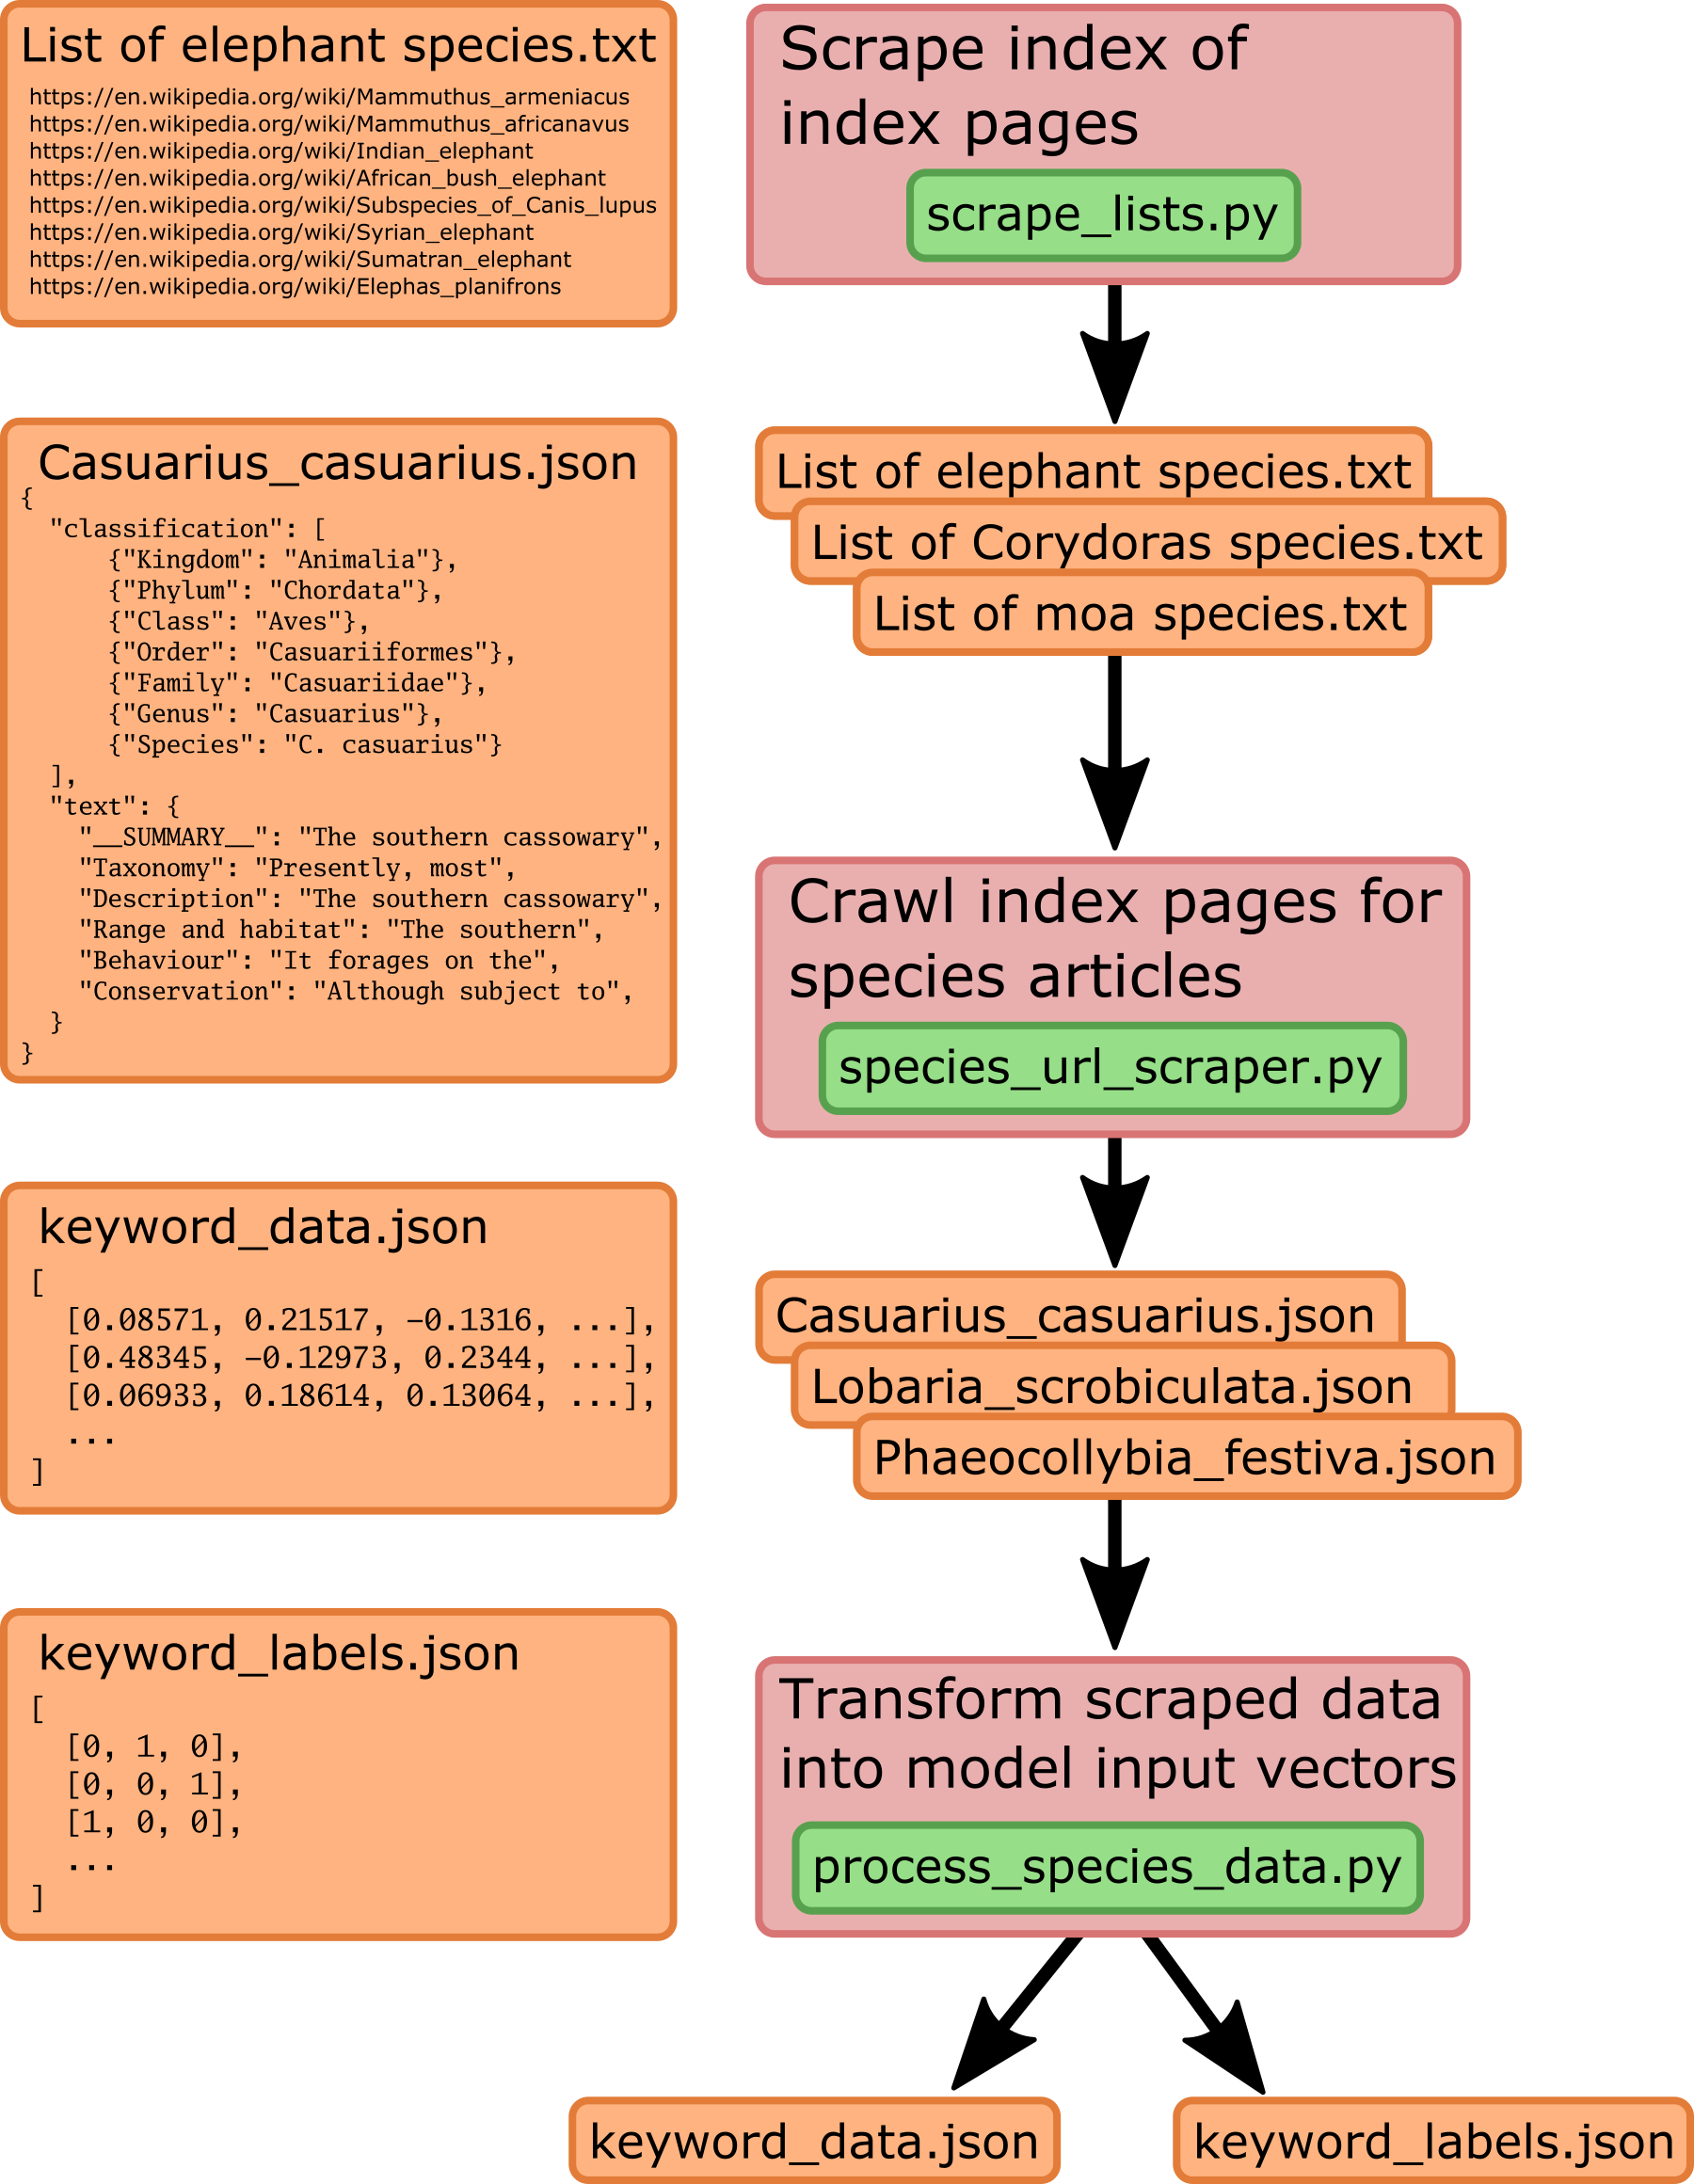
\includegraphics[width=\linewidth]{data.png}
  \caption{Visualization of the data-processing pipeline.}
  \label{fig:data}
\end{figure}

A flowchart of the data collection and processing pipeline can be seen in Figure \ref{fig:data}. The process involves collecting data from Wikipedia and then processing it into representations that will be used as inputs for the deep learning model.

\subsection{Scrape index pages}
The first step is to creates lists of species articles which is done by supplying manually-found species index pages using \texttt{species\_url\_scraper.py} which then scrapes these articles to output lists of Wikipedia article URLs.

\subsection{Scrape species articles} The next step consumes these lists and scrapes the Wikipedia pages themselves to extract the scientific classification as well as the text content from each of the sections.


\section{Methods}

These are the methods.

\section{Experiments}

These are the experiments.

\section{Results}

These are the results.

\section{Conclusions}

This is wonderful.

{\small
\bibliographystyle{ieee}
\bibliography{bibliography}
}

\end{document}
